\section{Testing finale}

\begin{frame}{Test Classe Category}
    \framesubtitle{Test di classe}
    
    \begin{figure}
        \centering
       % \includegraphics[width=.8\textwidth]{initial testing/testCategoria.png}
    \end{figure}    

    \note{
        Abbiamo scelto di effettuare a seguito del refactoring gli stessi test effettuati sulla versione 5, in modo da verificare che le funzionalità corrette dell'applicazione rimanessero tali anche dopo il refactoring.\\\bigskip
        
    }
\end{frame}

\begin{frame}{Test Classe Time}
    \framesubtitle{Test di requisiti e funzionalità}
    
    \begin{figure}
        \centering
        %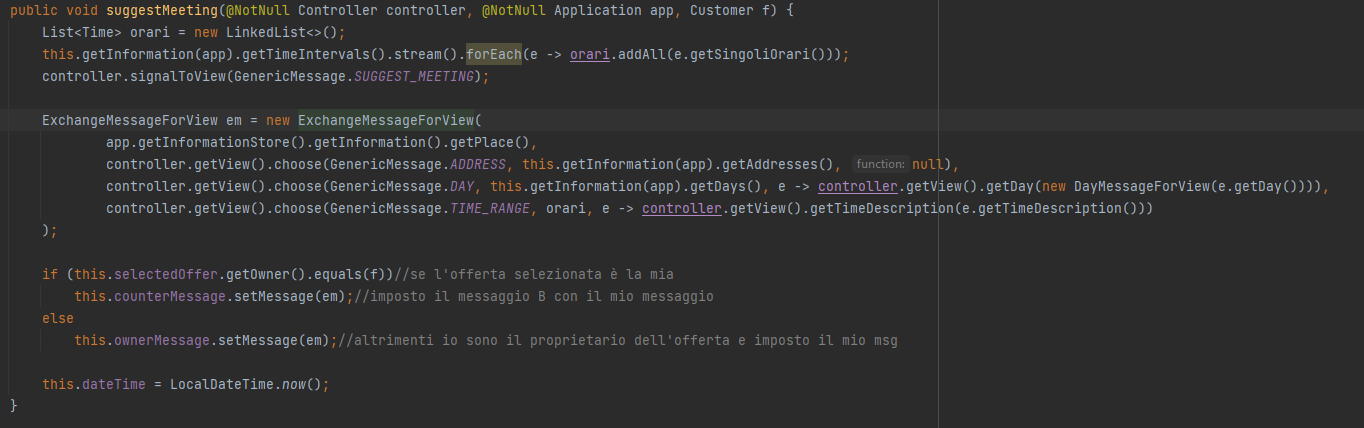
\includegraphics[width=.8\textwidth]{final testing/suggestMeeting classe Exchange.png}
    \end{figure}    

    \note{
        Per il test delle funzionalità abbiamo mantenuto la scelta della funzionalità individuata per il testing iniziale:\\
        ``Gli orari per effettuare lo scambio possono essere solo allo scoccare dell'ora o alla mezza (ogni trenta minuti)''\\\bigskip
        
        
    }

\end{frame}